\chapter{Ai4k8s System Design}
\label{ch:design}

This chapter describes the design of the Ai4k8s platform. Section~\ref{sec:design-goals}
states the design goals. Section~\ref{sec:arch-overview} presents the overall
architecture. Sections~\ref{sec:enforcement}--\ref{sec:mcda-layer} detail the three
layers of the Ai4k8s decision pipeline. Section~\ref{sec:local-llm} describes the
local LLM deployment. Section~\ref{sec:monitoring} covers the predictive monitoring
subsystem. Section~\ref{sec:web-mcp} describes the web interface and MCP server.

% -----------------------------------------------------------------------
\section{Design Goals}
\label{sec:design-goals}

The design of Ai4k8s is guided by five goals:

\begin{enumerate}
  \item \textbf{Predictive.} Autoscaling decisions should incorporate a forecast
  of near-future load, not only current metrics, to provision capacity ahead of
  demand.

  \item \textbf{Multi-criteria.} Decisions should balance cost, performance,
  stability, and forecast alignment simultaneously, rather than optimizing a
  single threshold.

  \item \textbf{Explainable.} Every scaling action must be accompanied by a
  human-readable justification that can be logged, audited, and presented to
  an operator.

  \item \textbf{Safe.} The system must never issue scaling recommendations that
  are physically impossible (e.g., scale above \texttt{maxReplicas}) or
  operationally unsafe (e.g., scale up when CPU is already low). A hard-coded
  enforcement layer provides this guarantee independently of the AI components.

  \item \textbf{On-premises first.} The system should operate entirely
  on-premises without cloud API dependency at idle, to support privacy-sensitive
  and air-gapped deployments. Cloud fallback is acceptable under resource
  contention.
\end{enumerate}

% -----------------------------------------------------------------------
\section{Architecture Overview}
\label{sec:arch-overview}

Figure~\ref{fig:arch} shows the high-level architecture of Ai4k8s. The platform
consists of four subsystems:

\begin{itemize}
  \item \textbf{Web application} (\texttt{ai\_kubernetes\_web\_app.py}): a
  Flask + SocketIO server exposing a real-time dashboard and REST API on port 5003.
  It orchestrates all subsystems and pushes live events to connected browsers.

  \item \textbf{MCP server} (\texttt{mcp\_http\_server.py}): a FastAPI server
  on port 5002 (localhost-only) that exposes Kubernetes operations as \gls{MCP}
  tools. The web application proxies all \texttt{kubectl} operations through it,
  isolating cluster access behind a structured API.

  \item \textbf{Ai4k8s autoscaling engine}: the predictive autoscaling subsystem,
  described in Sections~\ref{sec:enforcement}--\ref{sec:mcda-layer}.

  \item \textbf{Predictive monitoring subsystem}: the metrics collection and
  forecasting subsystem, described in Section~\ref{sec:monitoring}.
\end{itemize}

The component dependency graph is:
\begin{center}
\texttt{Browser $\leftrightarrow$ Flask+SocketIO $\to$ AutoscalingIntegration
$\to$ PredictiveAutoscaler $\to$ LLMAdvisor + MCDAOptimizer}
\end{center}

\begin{figure}[h]
  \centering
  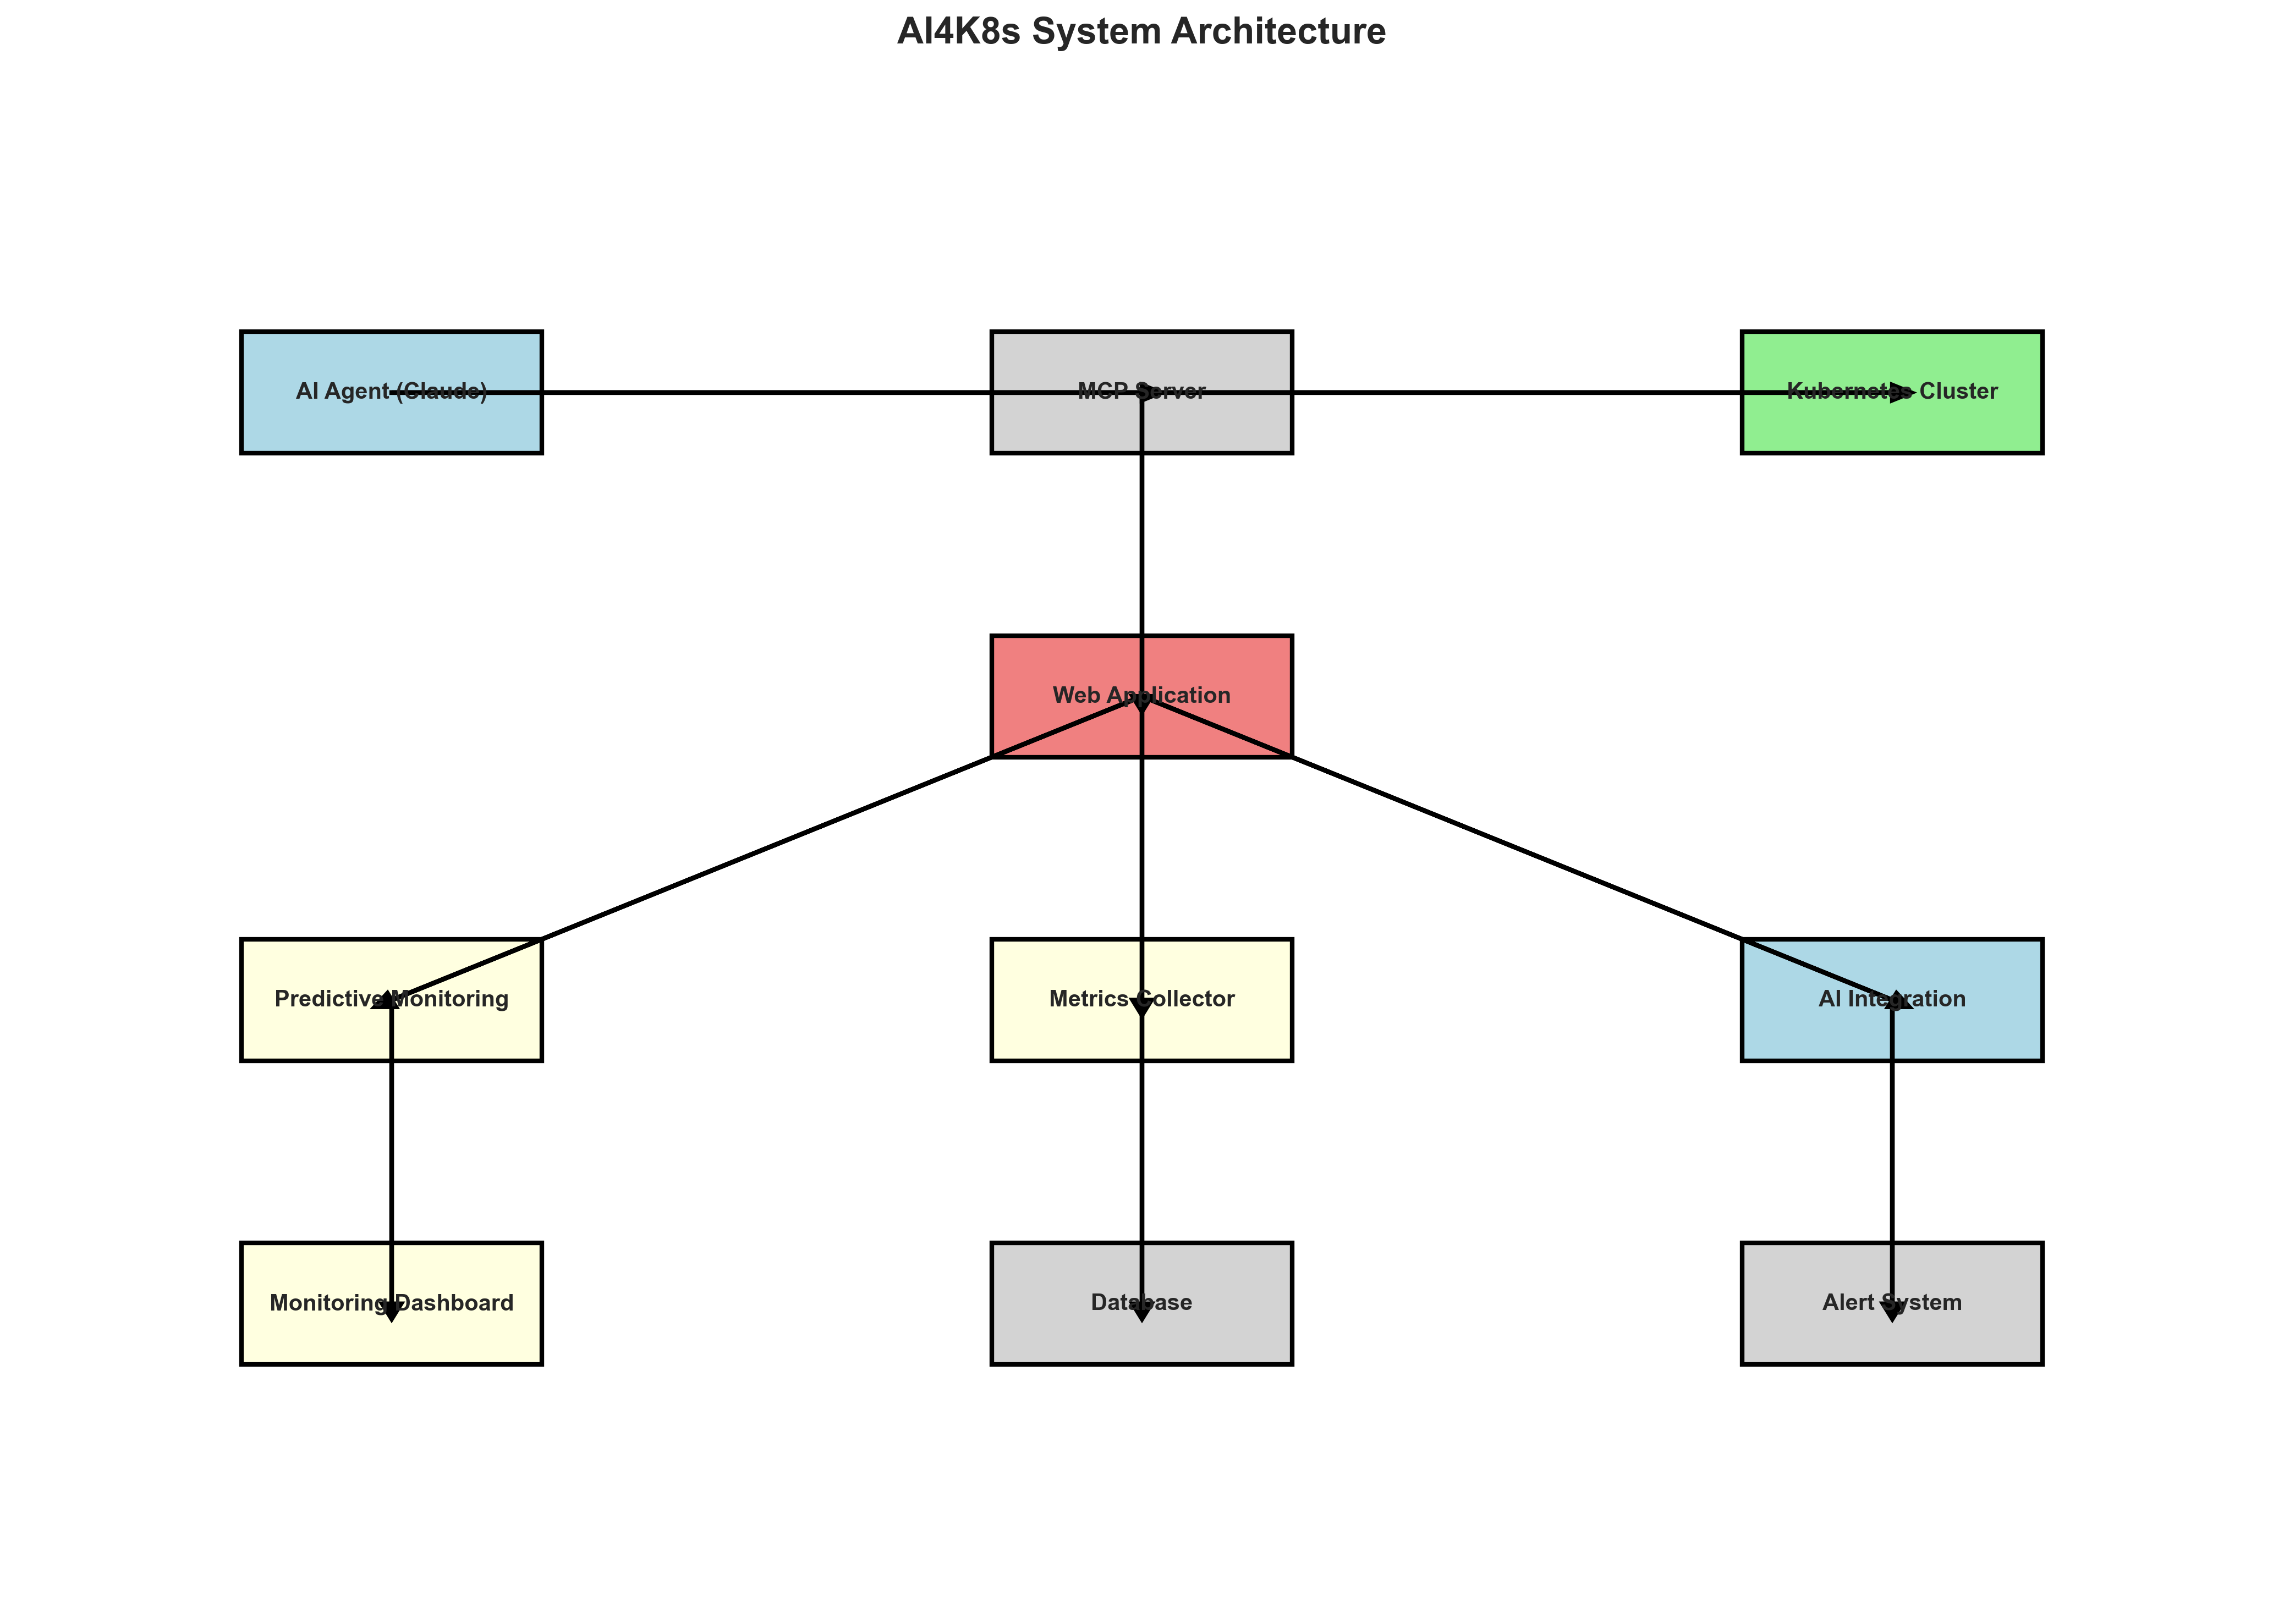
\includegraphics[width=0.92\linewidth]{images/figures/system_architecture}
  \caption{High-level architecture of Ai4k8s. The web application (port 5003)
    orchestrates the autoscaling engine, MCP server (port 5002), and monitoring
    subsystem. Kubernetes operations flow exclusively through the MCP tool layer.}
  \label{fig:arch}
\end{figure}

% -----------------------------------------------------------------------
\section{The Ai4k8s Decision Pipeline}
\label{sec:pipeline}

Ai4k8s implements a three-layer pipeline for every autoscaling decision.
The layers execute sequentially; each layer may short-circuit the pipeline
and return a final decision without consulting the subsequent layers.

\subsection{Enforcement Layer}
\label{sec:enforcement}

The enforcement layer applies hard safety rules before any model is consulted.
Rules are deterministic and do not depend on LLM or MCDA output:

\begin{itemize}
  \item If the requested action is \texttt{scale\_up} but CPU is below a
  configurable low-load threshold (default 30\%), the action is overridden to
  \texttt{maintain}. This prevents the LLM from recommending scale-up at idle
  based on stale or hallucinated context.

  \item If the target replica count would exceed \texttt{maxReplicas} or fall
  below \texttt{minReplicas}, it is clamped to the boundary.

  \item If the deployment annotation specifies a stateful service, any HPA
  scale-up recommendation is converted to a VPA right-sizing recommendation.

  \item If cluster-wide node pressure (CPU, memory, or disk) is detected,
  scale-up actions are blocked to avoid worsening an already-saturated node.
\end{itemize}

The enforcement layer runs synchronously and completes in under 1~ms. Its output
is logged with the reason string (e.g., \texttt{"CPU=12.1\% < threshold;
scale\_up overridden to maintain"}) as part of the decision trace.

\subsection{LLM Reasoning Layer}
\label{sec:llm-layer}

The LLM reasoning layer provides the semantic understanding component of the
pipeline. It receives a structured prompt containing:

\begin{itemize}
  \item Current CPU utilization, memory usage, and replica count for the target
  deployment.
  \item A 24-hour time-series trend summary (rising / stable / falling).
  \item A short-horizon forecast (next 5 minutes, produced by the predictive
  monitoring subsystem).
  \item The deployment's state-management annotation (\texttt{stateless} /
  \texttt{stateful}).
  \item The current HPA \texttt{minReplicas} and \texttt{maxReplicas}.
\end{itemize}

The model is instructed to return a JSON object with three fields:
\texttt{action} (\texttt{scale\_up} / \texttt{maintain} / \texttt{scale\_down}),
\texttt{target\_replicas} (integer), and \texttt{reasoning} (a one-sentence
explanation). The use of structured output mode eliminates parsing ambiguity.

\subsubsection{LLM Cascade}
\label{sec:cascade}

A resilient cascade chains three inference backends in order:

\begin{enumerate}
  \item \textbf{GPT-OSS (local Ollama/Qwen)}: attempted first. A thread-based
  soft timeout (default 90~s) prevents the main autoscaling loop from blocking
  indefinitely when Ollama is CPU-starved.

  \item \textbf{Groq (cloud)}: activated if the local model exceeds the soft
  timeout. Groq's \textit{llama-3.1-8b-instant} model returns a response in
  under 2~s.

  \item \textbf{Regex fallback}: activated if both LLM backends fail. A
  rule-based parser reads the raw CPU value and returns a safe default
  (\texttt{maintain} at current replicas).
\end{enumerate}

The cascade degrades gracefully rather than failing: even if both LLM backends
are unavailable, the enforcement layer and regex fallback together ensure a
safe, deterministic outcome.

\subsection{MCDA Optimization Layer}
\label{sec:mcda-layer}

The MCDA layer uses TOPSIS (Section~\ref{sec:topsis}) to score a set of candidate
replica counts across five criteria. Table~\ref{tab:mcda-criteria} describes each
criterion; Table~\ref{tab:mcda-weights} shows the four weight profiles.

\paragraph{Alternative Generation.}
Given the current replica count $r$, the module generates candidates
$r + \delta$ for $\delta \in \{-2,-1,0,+1,+2,+3\}$, plus
$r_{\min}$, $r_{\max}$, and an ``ideal'' count that would yield
70\% CPU utilization. Candidates outside $[r_{\min}, r_{\max}]$ are discarded,
producing 5--8 feasible alternatives.

\begin{table}[h]
  \centering
  \caption{MCDA criteria evaluated per alternative.}
  \label{tab:mcda-criteria}
  \small
  \begin{tabular}{llp{5.5cm}}
    \toprule
    Criterion & Type & Description \\
    \midrule
    Cost             & Cost    & Normalized replica count $r / r_{\max}$ \\
    Performance      & Benefit & Proximity of estimated CPU to 70\% sweet spot \\
    Stability        & Benefit & Penalizes large replica changes and contra-trend scaling \\
    Forecast Align.  & Benefit & Estimated peak CPU in 50--75\% comfort zone \\
    Response Time    & Cost    & Current CPU as proxy for request latency \\
    \bottomrule
  \end{tabular}
\end{table}

\begin{table}[h]
  \centering
  \caption{MCDA weight profiles ($\sum w_j = 1.0$). Default: balanced.}
  \label{tab:mcda-weights}
  \small
  \begin{tabular}{lccccc}
    \toprule
    Profile & Cost & Perf. & Stab. & Forec. & Resp. \\
    \midrule
    \textbf{Balanced (default)} & 0.20 & 0.30 & 0.25 & 0.15 & 0.10 \\
    Performance-first           & 0.10 & 0.40 & 0.15 & 0.20 & 0.15 \\
    Cost-optimized              & 0.40 & 0.20 & 0.20 & 0.10 & 0.10 \\
    Stability-first             & 0.15 & 0.20 & 0.40 & 0.15 & 0.10 \\
    \bottomrule
  \end{tabular}
\end{table}

The TOPSIS computation (Equations~\ref{eq:topsis-norm}--\ref{eq:topsis-closeness})
is deterministic and runs in under 1~ms. The per-alternative closeness coefficients
$C_i$, the selected action, and the dominance margin are appended to the decision
trace alongside the LLM reasoning string. If the TOPSIS closeness of the MCDA-optimal
action exceeds the LLM-recommended action by more than $\delta = 0.15$, MCDA overrides
the LLM and the override is logged with the gap value.

The decision trace for a single scaling event is:
\begin{verbatim}
{
  "deployment": "ingest",
  "enforcement": "pass (CPU=49.1% > threshold)",
  "llm_action": "scale_up",
  "llm_target": 3,
  "llm_reasoning": "Forecast shows rapidly_increasing trend...",
  "mcda_action": "maintain",
  "mcda_gap": 0.2585,
  "mcda_agreement": "override",
  "final_action": "maintain",
  "final_target": 2
}
\end{verbatim}

% -----------------------------------------------------------------------
\section{Local LLM Deployment}
\label{sec:local-llm}

Ai4k8s uses Ollama~\cite{ollama2023} to serve the local LLM. Ollama provides a
lightweight HTTP server that loads GGUF models from disk, manages model lifecycle,
and exposes both an OpenAI-compatible REST API (\texttt{/v1/chat/completions})
and a native API (\texttt{/api/chat}).

A key implementation detail is the handling of Qwen's chain-of-thought mode.
The Qwen3 family uses \textit{thinking} by default: the model writes its internal
reasoning to a hidden buffer before producing the visible response. When called
through the OpenAI-compatible endpoint, this causes the visible response to be
empty (the thinking tokens are consumed internally but not returned). Ai4k8s
detects the Ollama base URL at runtime and routes requests through the native
\texttt{/api/chat} endpoint with \texttt{"think": false}, bypassing the
chain-of-thought path and returning the answer directly.

\subsection{Model Selection}
\label{sec:model-selection}

Three models were evaluated for local inference (Table~\ref{tab:model-sizes}).
The final selection, \textit{qwen3:0.6b} (Q4, 522~MB), achieves 1.7~s idle
inference on a 4-vCPU VM. Under CPU-saturating muBench load the model exceeds
the 90~s soft timeout and falls back to Groq; this is a hardware constraint
rather than a model deficiency. The choice was driven by three factors:
inference speed at idle ($<$2~s), valid structured JSON output, and memory
footprint compatible with the 14~GiB VM running 12 active pods.

% -----------------------------------------------------------------------
\section{Predictive Monitoring Subsystem}
\label{sec:monitoring}

The predictive monitoring subsystem runs as a background thread and feeds the
LLM reasoning layer with current metrics and short-horizon forecasts.

\subsection{Metrics Collection}
\label{sec:metrics-collection}

Metrics are collected from the Kubernetes Metrics API via \texttt{kubectl top pods}
every $\Delta t = 300$~s per deployment, using a three-source fallback chain:
(1)~\texttt{kubectl top} (primary), (2)~Metrics API \texttt{v1beta1}, and
(3)~Kubelet Summary API. Individual requests that exceed a 10~s timeout trigger
the next source in the chain.

Raw CPU and memory values are normalized to utilization percentages:
\begin{equation}
  \mathrm{CPU\%} = \frac{\text{usage (millicores)}}{\text{allocatable (millicores)}}
  \times 100,
  \label{eq:cpu-norm}
\end{equation}
and analogously for memory. Each observation is appended to a 288-sample
(24-hour) ring buffer stored in memory.

\subsection{Time-Series Forecasting}
\label{sec:forecasting-impl}

The ring buffer feeds a one-step-ahead ARIMA$(p,d,q)$ model~\cite{box1970arima},
where the parameters $p=3$ (autoregressive order), $d=0$ (differencing), and
$q=0$ (moving average) are selected by grid-search over the muBench workload.
Each cycle produces a $h$-step-ahead point forecast $\hat{y}(t+h)$ and a trend
label (\textit{rising} / \textit{stable} / \textit{falling}) for the LLM prompt.

\subsection{Bootstrap Uncertainty Quantification}
\label{sec:uq}

Point forecasts alone do not express how much trust should be placed in a
prediction. Ai4k8s wraps every forecast in a \emph{prediction interval}
produced by nonparametric bootstrap resampling~\cite{efron1993introduction}.

$B = 50$ bootstrap samples of size $N$ are drawn with replacement from the
ring buffer. For each replicate $b \in \{1,\ldots,B\}$, a model is fitted and
$h$-step predictions $\hat{y}^{(b)}(t+h)$ are generated.

The \emph{epistemic} (model) uncertainty at horizon $h$ is:
\begin{equation}
  \sigma^{2}_{\mathrm{epi}}(h)
    = \frac{1}{B}\sum_{b=1}^{B}
      \bigl(\hat{y}^{(b)}(t+h) - \bar{y}(t+h)\bigr)^{2},
  \label{eq:epistemic}
\end{equation}
where $\bar{y}(t+h) = \frac{1}{B}\sum_{b}\hat{y}^{(b)}(t+h)$ is the mean
bootstrap forecast. The total predictive variance grows with horizon:
\begin{equation}
  \sigma^{2}(h)
    = \sigma^{2}_{\mathrm{ale}}\cdot\sqrt{h}
    + \sigma^{2}_{\mathrm{epi}}\cdot h,
  \label{eq:total-var}
\end{equation}
where $\sigma^{2}_{\mathrm{ale}}$ denotes the aleatoric (observation noise)
variance. This formulation models both noise accumulation ($\sqrt{h}$ term) and
model-uncertainty growth (linear term).

A $100(1-\alpha)\%$ prediction interval is then:
\begin{equation}
  \hat{y}(t+h) \pm z_{\alpha/2}\,\sigma(h),
  \label{eq:pred-interval}
\end{equation}
where $z_{\alpha/2}$ is the standard normal quantile ($z_{0.025}=1.96$ for
$95\%$). In addition, exceedance probabilities for four utilization thresholds
$\tau \in \{50, 70, 80, 90\}\%$ are computed as
$\Pr(\hat{y}(t+h) > \tau)$ using the complementary \gls{CDF} of
$\mathcal{N}(\hat{y}(t+h),\,\sigma^{2}(h))$.

\begin{figure}[h]
  \centering
  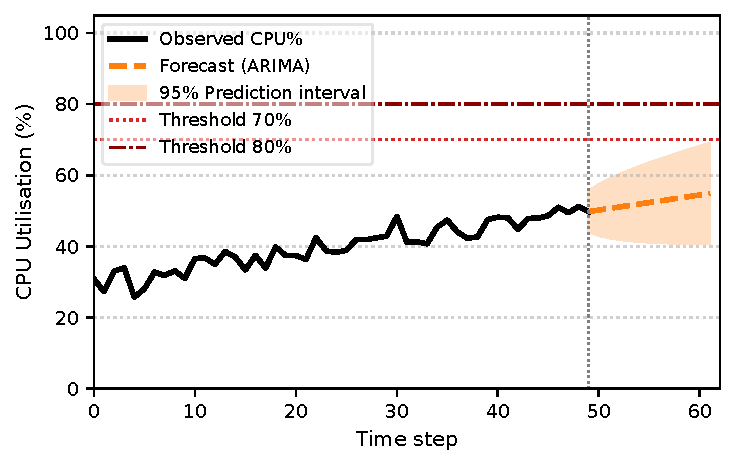
\includegraphics[width=0.92\linewidth]{images/figures/fig_forecast_uq}
  \caption{Example ARIMA forecast with 95\% bootstrap prediction interval
    (Equations~\ref{eq:epistemic}--\ref{eq:pred-interval}) on a rising CPU trace.
    The shaded band widens with horizon; threshold lines mark the 70\% and 80\%
    exceedance boundaries used for proactive alerting.}
  \label{fig:forecast-uq}
\end{figure}

\subsection{Calibrated Anomaly Detection}
\label{sec:anomaly}

An Isolation Forest~\cite{liu2008isolation} with contamination $c=0.1$ produces
a raw score $s \in [-1,1]$ for each observation. Raw scores are not directly
interpretable as probabilities; Ai4k8s applies \emph{Platt scaling} to obtain
a calibrated anomaly probability:
\begin{equation}
  \Pr(\text{anomaly} \mid s)
    = \sigma(As + B)
    = \frac{1}{1 + e^{-(As + B)}},
  \label{eq:platt}
\end{equation}
with calibration parameters $A = -5.0$ and $B = -0.5$. Observations with
$\Pr(\text{anomaly}) \ge 0.5$ are flagged in the LLM prompt as anomalous.

Detection confidence quantifies how far the probability is from maximum
uncertainty:
\begin{equation}
  \gamma = 2\,\bigl|\Pr(\text{anomaly}) - 0.5\bigr| \in [0,1].
  \label{eq:confidence}
\end{equation}
$\gamma \approx 1$ indicates high confidence ($\Pr$ near 0 or 1); $\gamma \approx 0$
indicates an uncertain detection near the decision boundary.

% -----------------------------------------------------------------------
\section{Web Interface and MCP Server}
\label{sec:web-mcp}

The Ai4k8s web interface provides a real-time dashboard with four views:
cluster status (pod list with live CPU/memory bars), autoscaling decisions
(timestamped log of Ai4k8s actions with full decision traces), anomaly timeline,
and LLM chat (direct natural-language queries to the cluster via the MCP tool
server).

The \gls{MCP} server exposes twelve Kubernetes operations as typed tool calls,
including \texttt{list\_pods}, \texttt{get\_pod\_logs}, \texttt{scale\_deployment},
and \texttt{get\_metrics}. All cluster mutations flow through MCP, providing a
single auditable interface for both the Ai4k8s engine and the interactive chat
client.
